\documentclass[9pt,letter]{article}
\usepackage{lmodern}
\usepackage{amssymb,amsmath}
\usepackage{ifxetex,ifluatex}
\usepackage{fixltx2e} % provides \textsubscript
\ifnum 0\ifxetex 1\fi\ifluatex 1\fi=0 % if pdftex
  \usepackage[T1]{fontenc}
  \usepackage[utf8]{inputenc}
\else % if luatex or xelatex
  \ifxetex
    \usepackage{mathspec}
  \else
    \usepackage{fontspec}
  \fi
  \defaultfontfeatures{Ligatures=TeX,Scale=MatchLowercase}
\fi
% use upquote if available, for straight quotes in verbatim environments
\IfFileExists{upquote.sty}{\usepackage{upquote}}{}
% use microtype if available
\IfFileExists{microtype.sty}{%
\usepackage{microtype}
\UseMicrotypeSet[protrusion]{basicmath} % disable protrusion for tt fonts
}{}
\usepackage[margin=.75in]{geometry}
\usepackage{hyperref}
\hypersetup{unicode=true,
            pdftitle={Assignment 4},
            pdfauthor={Azoacha Forcheh, 20558994},
            pdfborder={0 0 0},
            breaklinks=true}
\urlstyle{same}  % don't use monospace font for urls
\usepackage{color}
\usepackage{fancyvrb}
\newcommand{\VerbBar}{|}
\newcommand{\VERB}{\Verb[commandchars=\\\{\}]}
\DefineVerbatimEnvironment{Highlighting}{Verbatim}{commandchars=\\\{\}}
% Add ',fontsize=\small' for more characters per line
\usepackage{framed}
\definecolor{shadecolor}{RGB}{248,248,248}
\newenvironment{Shaded}{\begin{snugshade}}{\end{snugshade}}
\newcommand{\KeywordTok}[1]{\textcolor[rgb]{0.13,0.29,0.53}{\textbf{#1}}}
\newcommand{\DataTypeTok}[1]{\textcolor[rgb]{0.13,0.29,0.53}{#1}}
\newcommand{\DecValTok}[1]{\textcolor[rgb]{0.00,0.00,0.81}{#1}}
\newcommand{\BaseNTok}[1]{\textcolor[rgb]{0.00,0.00,0.81}{#1}}
\newcommand{\FloatTok}[1]{\textcolor[rgb]{0.00,0.00,0.81}{#1}}
\newcommand{\ConstantTok}[1]{\textcolor[rgb]{0.00,0.00,0.00}{#1}}
\newcommand{\CharTok}[1]{\textcolor[rgb]{0.31,0.60,0.02}{#1}}
\newcommand{\SpecialCharTok}[1]{\textcolor[rgb]{0.00,0.00,0.00}{#1}}
\newcommand{\StringTok}[1]{\textcolor[rgb]{0.31,0.60,0.02}{#1}}
\newcommand{\VerbatimStringTok}[1]{\textcolor[rgb]{0.31,0.60,0.02}{#1}}
\newcommand{\SpecialStringTok}[1]{\textcolor[rgb]{0.31,0.60,0.02}{#1}}
\newcommand{\ImportTok}[1]{#1}
\newcommand{\CommentTok}[1]{\textcolor[rgb]{0.56,0.35,0.01}{\textit{#1}}}
\newcommand{\DocumentationTok}[1]{\textcolor[rgb]{0.56,0.35,0.01}{\textbf{\textit{#1}}}}
\newcommand{\AnnotationTok}[1]{\textcolor[rgb]{0.56,0.35,0.01}{\textbf{\textit{#1}}}}
\newcommand{\CommentVarTok}[1]{\textcolor[rgb]{0.56,0.35,0.01}{\textbf{\textit{#1}}}}
\newcommand{\OtherTok}[1]{\textcolor[rgb]{0.56,0.35,0.01}{#1}}
\newcommand{\FunctionTok}[1]{\textcolor[rgb]{0.00,0.00,0.00}{#1}}
\newcommand{\VariableTok}[1]{\textcolor[rgb]{0.00,0.00,0.00}{#1}}
\newcommand{\ControlFlowTok}[1]{\textcolor[rgb]{0.13,0.29,0.53}{\textbf{#1}}}
\newcommand{\OperatorTok}[1]{\textcolor[rgb]{0.81,0.36,0.00}{\textbf{#1}}}
\newcommand{\BuiltInTok}[1]{#1}
\newcommand{\ExtensionTok}[1]{#1}
\newcommand{\PreprocessorTok}[1]{\textcolor[rgb]{0.56,0.35,0.01}{\textit{#1}}}
\newcommand{\AttributeTok}[1]{\textcolor[rgb]{0.77,0.63,0.00}{#1}}
\newcommand{\RegionMarkerTok}[1]{#1}
\newcommand{\InformationTok}[1]{\textcolor[rgb]{0.56,0.35,0.01}{\textbf{\textit{#1}}}}
\newcommand{\WarningTok}[1]{\textcolor[rgb]{0.56,0.35,0.01}{\textbf{\textit{#1}}}}
\newcommand{\AlertTok}[1]{\textcolor[rgb]{0.94,0.16,0.16}{#1}}
\newcommand{\ErrorTok}[1]{\textcolor[rgb]{0.64,0.00,0.00}{\textbf{#1}}}
\newcommand{\NormalTok}[1]{#1}
\usepackage{graphicx,grffile}
\makeatletter
\def\maxwidth{\ifdim\Gin@nat@width>\linewidth\linewidth\else\Gin@nat@width\fi}
\def\maxheight{\ifdim\Gin@nat@height>\textheight\textheight\else\Gin@nat@height\fi}
\makeatother
% Scale images if necessary, so that they will not overflow the page
% margins by default, and it is still possible to overwrite the defaults
% using explicit options in \includegraphics[width, height, ...]{}
\setkeys{Gin}{width=\maxwidth,height=\maxheight,keepaspectratio}
\IfFileExists{parskip.sty}{%
\usepackage{parskip}
}{% else
\setlength{\parindent}{0pt}
\setlength{\parskip}{6pt plus 2pt minus 1pt}
}
\setlength{\emergencystretch}{3em}  % prevent overfull lines
\providecommand{\tightlist}{%
  \setlength{\itemsep}{0pt}\setlength{\parskip}{0pt}}
\setcounter{secnumdepth}{0}
% Redefines (sub)paragraphs to behave more like sections
\ifx\paragraph\undefined\else
\let\oldparagraph\paragraph
\renewcommand{\paragraph}[1]{\oldparagraph{#1}\mbox{}}
\fi
\ifx\subparagraph\undefined\else
\let\oldsubparagraph\subparagraph
\renewcommand{\subparagraph}[1]{\oldsubparagraph{#1}\mbox{}}
\fi

%%% Use protect on footnotes to avoid problems with footnotes in titles
\let\rmarkdownfootnote\footnote%
\def\footnote{\protect\rmarkdownfootnote}

%%% Change title format to be more compact
\usepackage{titling}

% Create subtitle command for use in maketitle
\newcommand{\subtitle}[1]{
  \posttitle{
    \begin{center}\large#1\end{center}
    }
}

\setlength{\droptitle}{-2em}
  \title{Assignment 4}
  \pretitle{\vspace{\droptitle}\centering\huge}
  \posttitle{\par}
  \author{Azoacha Forcheh, 20558994}
  \preauthor{\centering\large\emph}
  \postauthor{\par}
  \date{}
  \predate{}\postdate{}

\usepackage{graphicx}
\usepackage{color}
\usepackage{enumitem}
\newcommand{\benum}{\begin{enumerate}}
\newcommand{\eenum}{\end{enumerate}}
\newcommand{\bitem}{\begin{itemize}}
\newcommand{\eitem}{\end{itemize}}

\begin{document}
\maketitle

\benum

\item 

Download the \texttt{olive} data from the course website. In that file,
there is a dataset on the fatty acid content of 572 different Italian
olive oils. In total eight different fatty acids are measured. All olive
oils come from one of nine different olive growing regions in Italy.

\begin{center}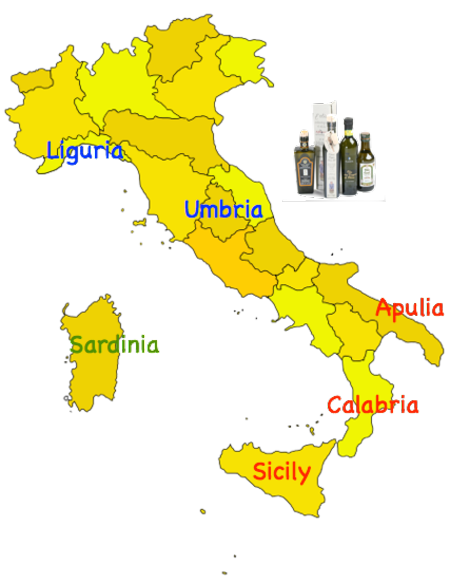
\includegraphics{a4_testing_files/figure-latex/unnamed-chunk-1-1} \end{center}

Once you load this file into your \texttt{R} session there will be a
data set called \texttt{olive}.

In this question you are going to focus on the fatty acid
\texttt{oleic}.

\benum
\item (2 marks) Separate the data on \texttt{oleic} into 9 different
groups as defined by the olive growing \texttt{Area}, and draw side by
side boxplots of all 9 groups. Colour the boxplots uniquely using

\begin{Shaded}
\begin{Highlighting}[]
\KeywordTok{library}\NormalTok{(colorspace)}
\NormalTok{cols <-}\StringTok{ }\KeywordTok{rainbow_hcl}\NormalTok{(}\DecValTok{9}\NormalTok{) }\CommentTok{# Use these colours.}
\end{Highlighting}
\end{Shaded}

Show your code together with your output.

\begin{Shaded}
\begin{Highlighting}[]
\NormalTok{groups =}\StringTok{ }\KeywordTok{with}\NormalTok{(olive, }\KeywordTok{split}\NormalTok{(oleic, Area))}
\NormalTok{size_ord =}\StringTok{ }\KeywordTok{order}\NormalTok{(}\KeywordTok{sapply}\NormalTok{(groups, IQR))}
\NormalTok{ord =}\StringTok{ }\KeywordTok{names}\NormalTok{(groups)[size_ord]}
\KeywordTok{boxplot}\NormalTok{(groups[ord], }\DataTypeTok{col=}\NormalTok{cols[size_ord], }
        \DataTypeTok{main=}\StringTok{"Oleic Levels by Olive Growing Area"}\NormalTok{)}
\end{Highlighting}
\end{Shaded}

\begin{center}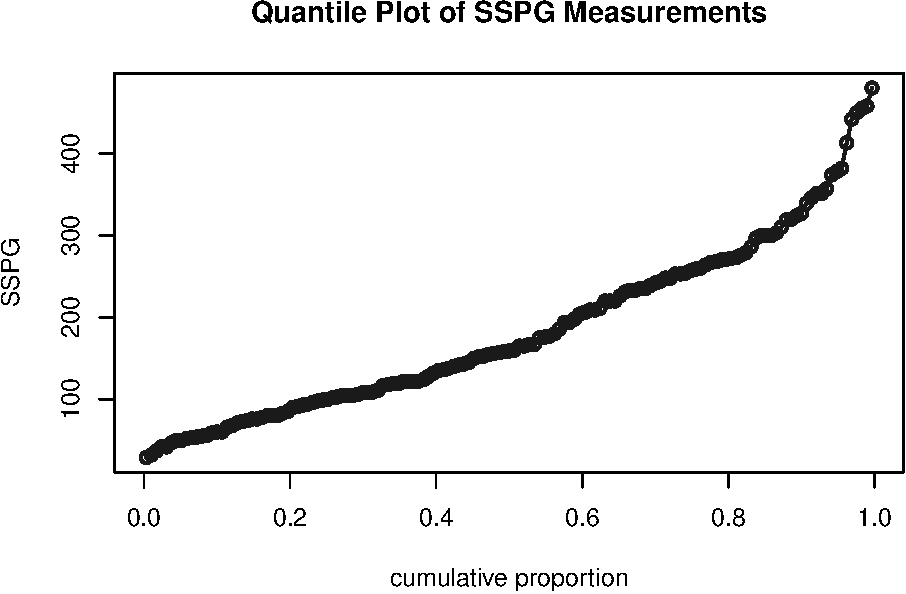
\includegraphics{a4_testing_files/figure-latex/unnamed-chunk-4-1} \end{center}

\item 

Load the \texttt{R} package \texttt{PairViz}. Use the variate
\texttt{oleic} and the same colours for the olive growing areas as in
part (a) throughout the following:

\benum
\item (3 marks) Suppose we wish every pair of boxplots to appear next to
one another in the same plot. \bitem
\item How many such pairwise comparisons exist?

\[
solution = 37 (need to explain why)
\]

\item 

Give the code that will construct this display (without any other
constraint on the ordering). \item Show the display which resulted from
your code.

\begin{Shaded}
\begin{Highlighting}[]
\CommentTok{# Make this bigger and shorten names}
\NormalTok{n =}\StringTok{ }\KeywordTok{length}\NormalTok{(groups)}
\NormalTok{ord =}\StringTok{ }\KeywordTok{eulerian}\NormalTok{(n)}
\KeywordTok{boxplot}\NormalTok{(groups[ord], }\DataTypeTok{col=}\NormalTok{cols[ord])}
\end{Highlighting}
\end{Shaded}

\begin{center}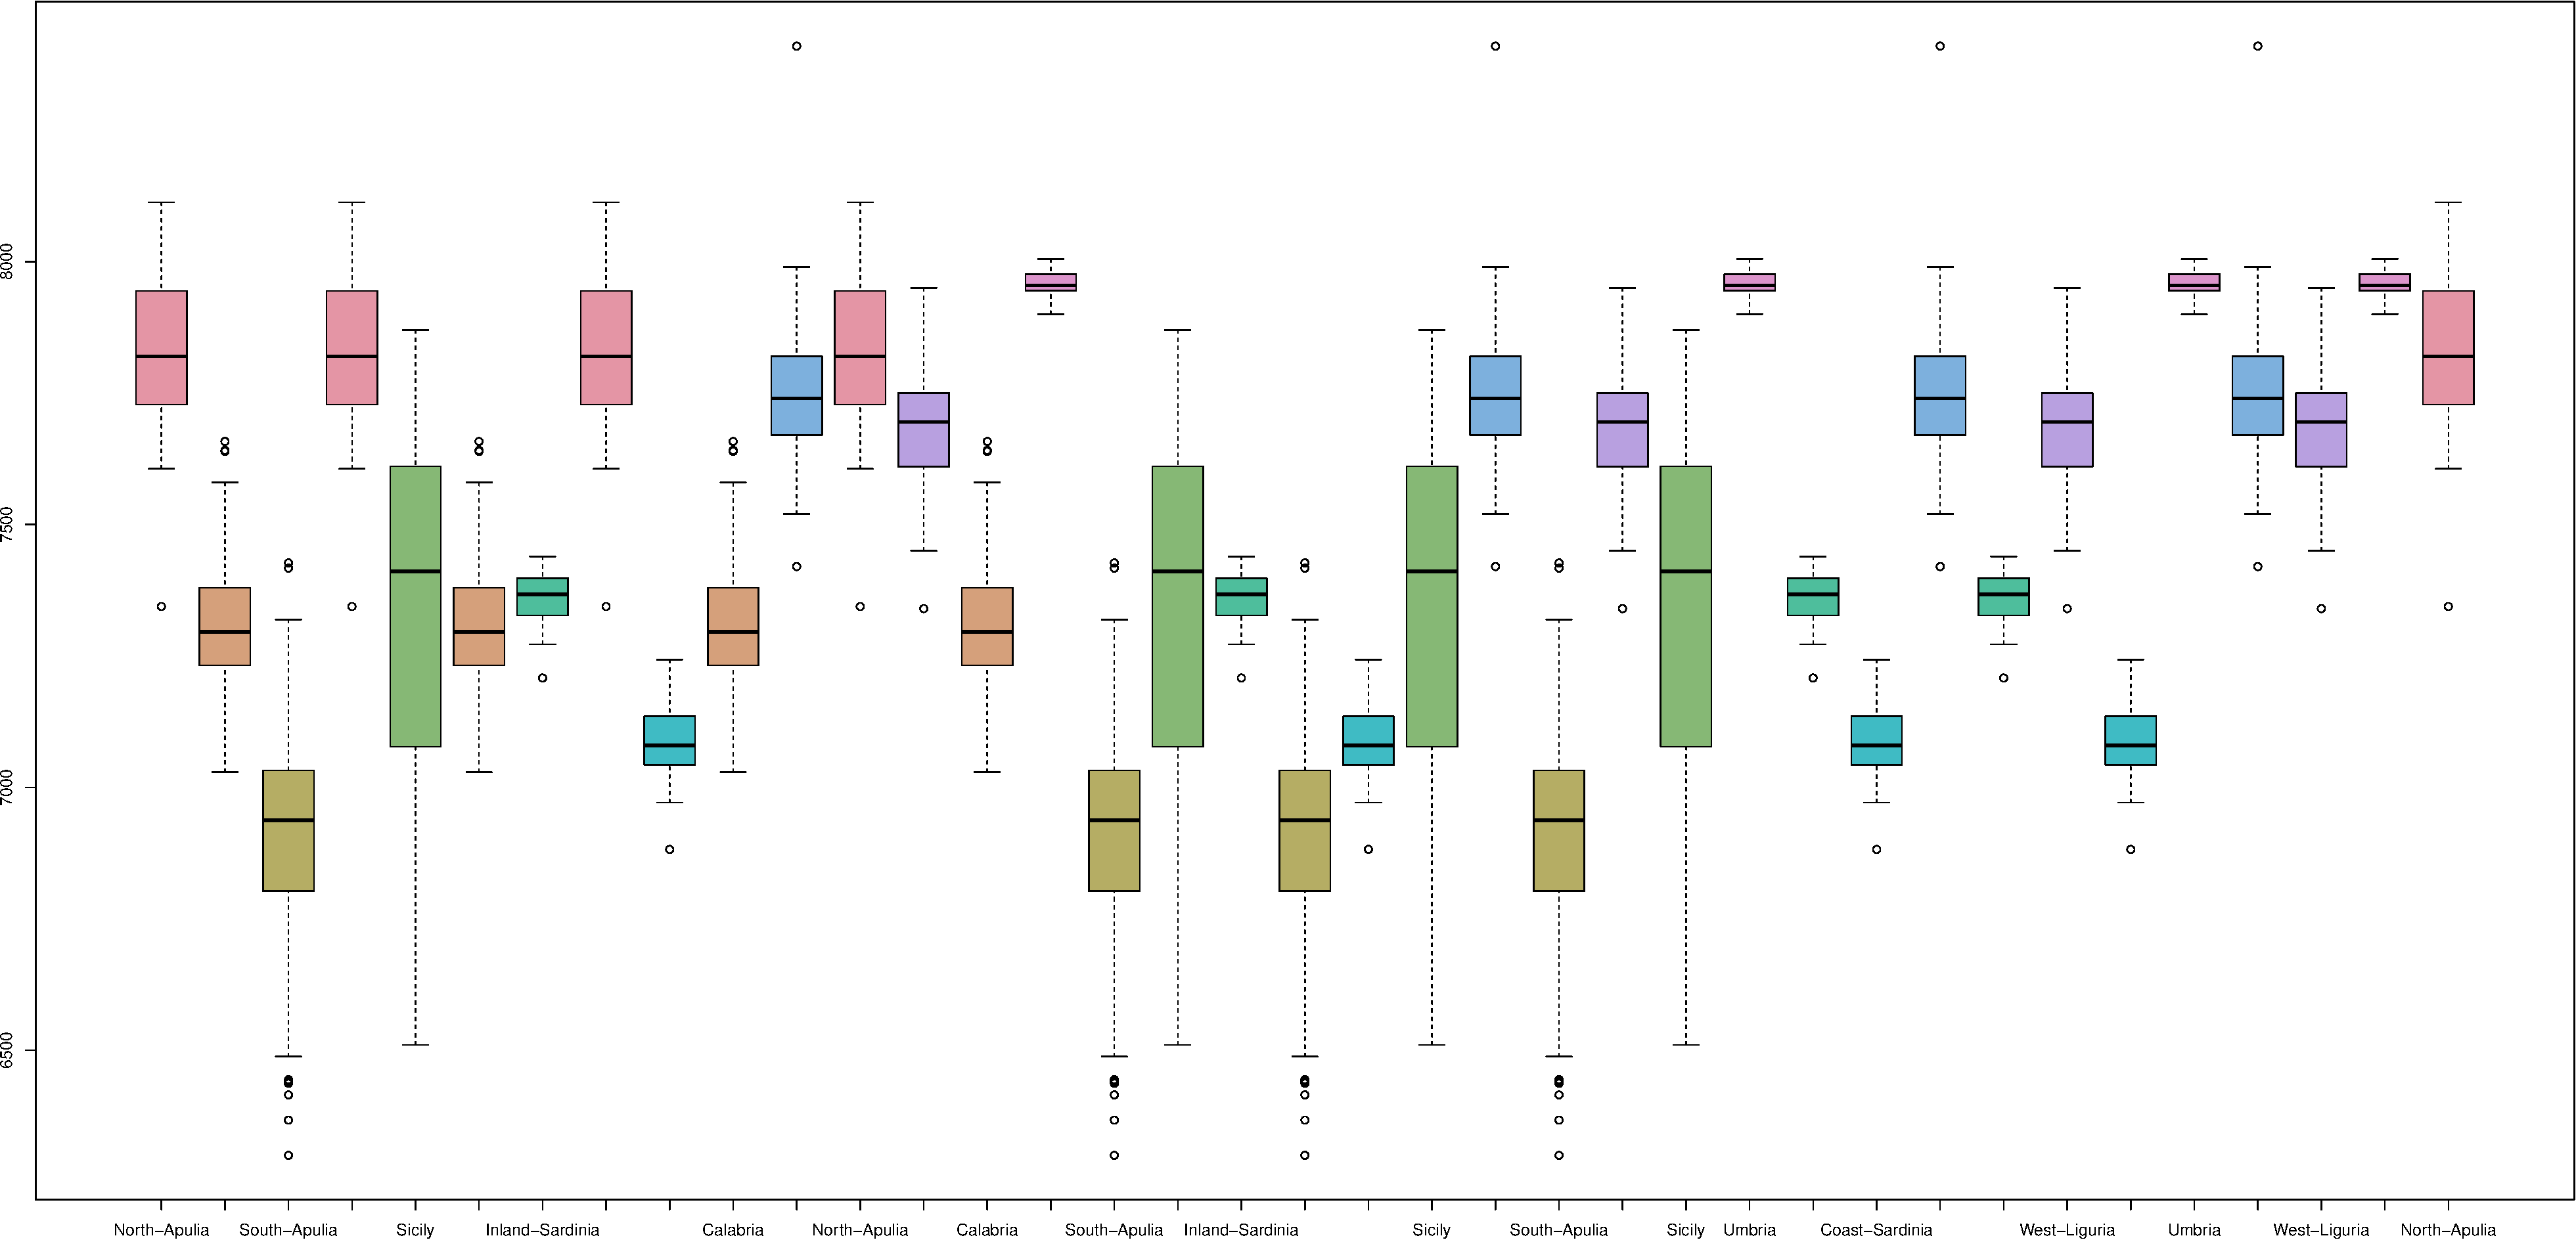
\includegraphics{a4_testing_files/figure-latex/unnamed-chunk-6-1} \end{center}

\eitem        

\item 

(5 marks) Suppose we wish every pair of boxplots to appear next to one
another in the same plot but that the boxplots should be grouped so that
all areas appear only once in each group. \bitem
\item Maintaining the same colours for the areas as before, give the
code that will construct this display (without any other constraint on
the ordering).\\
\item Show the display which resulted from your code. \eitem

\item 

(7 marks) Construct \(t\) tests for every pair of olive growing areas
(recall \texttt{pairwise.t.test} from class). Use the significance
levels from these tests to construct an ordering of the boxplot pairs,
one which favours having the most significantly different pairs at the
left of the display. \bitem
\item Show your code. \item Show the resulting display. \item Does the
ordering perfectly arrange the boxplots so that for any pairwise
comparison, those to the left are more significant and those to the
right are less significant? \item Explain why the ordering was
successful (or unsuccessful) in this way. \item Show a display showing
only the first 8 comparisons.

\eitem

\item 

(7 marks) Use the significance levels from part (iii) but now order the
boxplots so that the \textbf{least} significant differences appear
earliest in the sequence from left to right. \bitem
\item Show your code. \item Show the resulting display. \item Does the
ordering perfectly arrange the boxplots so that for any pairwise
comparison, those to the left are less significant and those to the
right are more significant? \item Explain why the ordering was
successful (or unsuccessful) in this way. \item Show a display showing
only the first 8 comparisons. \eitem

\item 

(2 marks) Is the sequence used in part (iii) the reverse of that in part
(iv)? \bitem
\item If it is, must it be the reverse?\\
\item If it is not, is it impossible for it to be the same?\\
\item Either way, explain your reasoning.\\
\eitem

\eenum

\item 

The olive growing areas are divided into three different regions: North,
South, and Sardinia. In this part of the question, interest lies only in
comparisons between each growing area in the south and each area in
Sardinia. That is, each southern area (4 areas) is to be compared to
each Sardinian area (2 areas) yielding a total of 8 comparisons of
interest.

\benum
\item (4 marks) Having loaded \texttt{PairViz}, create a graph having
all six areas in the South and Sardinia as nodes and with edges between
every pair whose comparison is of interest. \bitem
\item plot this graph \item show the code used to create the graph and
to plot it. \eitem

\item 

(4 marks) Using the graph from part (i), construct an Eulerian and use
that Eulerian to produce a sequence of boxplots that show the
comparisons of interest. \bitem
\item show the boxplot display \item show the code used to construct the
Eulerian and the display.\\
\eitem

\eenum
\eenum

\eenum


\end{document}
